% ============================================================================
% Chapitre 4 --- Implémentation
% ============================================================================
\chapter{Implémentation}
\label{chap:implementation}

\section{Organisation du dépôt}

\begin{lstlisting}[language={}, numbers=none, caption={Arborescence du dépôt.}]
backend/   sim.py        modèle de la ligne et KPI
           server.py     FastAPI : WebSocket /ws, REST /api/*
           storage.py    historique SQLite
frontend/  index.html, style.css
           js/app.js     tableau de bord, historique, commandes
           unity/        build WebGL (généré, non versionné)
unity/     projet Unity 6 (URP)
           Assets/Scripts/Net      client WebSocket, DTO du protocole
           Assets/Scripts/Scene    ligne, machines, caméra, étiquettes
           Assets/Scripts/Bench    banc d'essai des scénarios
           Assets/Editor           construction de la scène, build WebGL
tests/     test_sim.py   cohérence du modèle (21 tests)
           test_api.py   WebSocket et REST (2 tests)
tools/     resultats_vers_markdown.py   résultats du banc d'essai
docs/      rapport/, presentation/, repartition/, cahier-des-charges.md,
           protocole-websocket.md, resultats-unity.md, manuel-utilisateur.md
\end{lstlisting}

L'application se lance par une seule commande (\code{python backend/server.py}) puis s'ouvre à l'adresse \code{http://localhost:8000}. Le backend sert aussi les fichiers de l'interface et le build Unity WebGL~: aucun serveur web séparé n'est nécessaire. Les fichiers du build sont compressés (\code{.unityweb}, gzip)~; un petit intergiciel du backend ajoute l'en-tête \code{Content-Encoding} et le type \textsc{mime} adapté pour que le navigateur les décompresse lui-même. Une variable d'environnement facultative, \code{SIM\_SEED}, fixe la graine aléatoire pour rendre les pannes reproductibles.

\section{Le modèle de simulation (\code{sim.py})}

La classe \code{Sim} contient l'état de la ligne~: les files (\code{deque}), les machines de chaque poste (\code{Server}~: produit en cours, temps restant, drapeau \enquote{terminé}), les produits en transit et les compteurs statistiques. La boucle principale \code{step(dt)} applique les règles décrites au chapitre~\ref{chap:conception} (figure~\ref{fig:flux}). L'extrait suivant montre le cœur du traitement d'un poste~: libération du produit terminé si la file aval a de la place, sinon blocage~; puis prise d'un nouveau produit et avancement du traitement.

\begin{lstlisting}[language=Python, caption={Traitement des postes, de l'aval vers l'amont (\code{Sim.step}).}, label=lst:step]
limit = c["wip_limit"] if c["adaptive"] else c["buffer"]
for i in reversed(range(N)):
    for s in self.servers[i]:
        if s.done and not self._release(i, s, limit):
            self.blocked[i] += dt          # file aval pleine : poste bloqué
            continue
        if s.p is None and not self.down[i]:
            if i == 0:                     # alimentation : matière illimitée
                s.p = Product(self.next_id, t); self.next_id += 1
            elif self.queues[i]:
                p = self.queues[i].popleft()
                self.wait_sum[i] += t - p.t_enq
                s.p = p
            else:
                continue                   # poste en attente
            s.rem = c["times"][i]
        if s.p is not None and not s.done and not self.down[i]:
            s.rem -= dt; self.busy[i] += dt
            if s.rem <= 1e-9:
                s.done = True
                if i == CONTROLE:          # 5 % de rejets au contrôle
                    s.p.reject = self.rng.random() < c["reject_rate"]
                self._release(i, s, limit)
\end{lstlisting}

Le générateur aléatoire est propre à chaque simulation et initialisé par une graine~: deux simulations de même graine et de mêmes paramètres produisent exactement les mêmes pannes et les mêmes rejets. C'est la condition d'une comparaison honnête entre scénarios (chapitre~\ref{chap:optimisation}). La fonction \code{compare\_presets} exécute chaque scénario pendant une heure simulée, sans affichage, en moins de 0{,}1~s par scénario.

\section{Le backend (\code{server.py}, \code{storage.py})}

Le serveur FastAPI démarre une tâche asynchrone qui, toutes les 100~ms réelles, fait avancer la simulation du nombre de pas correspondant à la vitesse choisie ($\times$4 par défaut, soit 8 pas de 0{,}05~s), puis diffuse l'état à tous les navigateurs connectés. Plusieurs postes peuvent superviser la même ligne simultanément. Les commandes reçues sont validées (\code{\_station}, bornes des valeurs)~; une commande invalide renvoie un message \code{error}.

Le module \code{storage.py} enregistre l'historique dans trois tables SQLite~:
\begin{itemize}
  \item \code{runs}~: une ligne par exécution (démarrage, scénario appliqué, remise à zéro), avec la configuration~;
  \item \code{samples}~: un relevé des \ac{KPI} et de l'état des postes par minute simulée~;
  \item \code{events}~: pannes, remises en service et changements de réglages, transmis par un rappel (\code{on\_event}) que la simulation appelle à chaque événement.
\end{itemize}
La comparaison de scénarios, plus coûteuse, est exécutée dans un fil séparé (\code{asyncio.\allowbreak to\_thread}) pour ne pas interrompre la diffusion temps réel.

\section{La scène 3D (Unity)}

La scène est un projet \textbf{Unity~6} (pipeline URP, espace colorimétrique linéaire) construit uniquement à partir de primitives (boîtes, cylindres, sphères) et d'un maillage de trémie généré par code~: aucun modèle externe n'est importé. Un outil d'édition (menu \code{Twin > Construire la scène}) crée la scène, les matériaux et les textures de façon reproductible, ce qui évite de dépendre d'un fichier binaire modifié à la main. Chaque poste a une silhouette propre --- trémie pour l'alimentation, broche rotative pour le traitement, caméra et faisceau de balayage pour le contrôle, presse et carton pour l'emballage --- et porte un voyant aux couleurs des états de la figure~\ref{fig:etats}, une barre de progression et une étiquette flottante (nom, état, temps de cycle, file). Quand un poste passe à plusieurs machines, la scène ajoute les machines en parallèle et un aiguillage du convoyeur.

\begin{table}[H]
\centering
\caption{Scripts C\# de la scène Unity.}
\label{tab:scripts}
\small
\begin{tabularx}{\textwidth}{@{}l X@{}}
\toprule
\textbf{Script} & \textbf{Rôle} \\
\midrule
\code{TwinClient}, \code{WsTransport} & Connexion WebSocket (natif dans l'éditeur, passerelle JavaScript en WebGL), décodage des messages, tampon d'états \\
\code{LineController} & Applique l'état reçu~: machines, produits, palette, étiquettes de sortie \\
\code{LineBuilder}, \code{StationUnit} & Construction et animation des machines (broche, faisceau, presse, voyant, barre) \\
\code{OrbitCamera} & Caméra orbitale lissée, brouillard dépendant de la distance, retour à la vue globale \\
\code{WorldLabel} & Étiquettes TextMeshPro orientées vers la caméra \\
\code{LineBridge} & Pont page web $\leftrightarrow$ Unity (sélection d'une machine, vue globale) \\
\code{ScenarioBenchmark} & Banc d'essai~: joue chaque scénario et exporte les mesures \\
\bottomrule
\end{tabularx}
\end{table}

\begin{figure}[H]
\centering
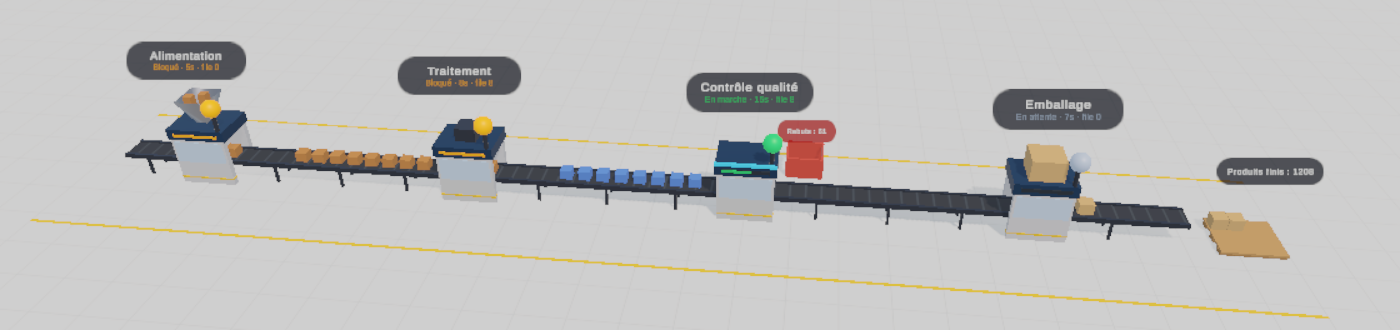
\includegraphics[width=\textwidth]{images/screenshots/vue_globale.png}
\caption{Vue d'ensemble de la scène Unity (build WebGL, ligne initiale). Les produits s'accumulent devant le contrôle qualité, le traitement et l'alimentation sont bloqués en amont~; le bac rouge reçoit les rebuts, la palette les produits finis.}
\label{fig:vue_globale}
\end{figure}

\subsection{Fluidité}

Les produits ne sont pas déplacés par un calcul propre à la scène~: le client conserve un tampon des derniers états reçus (10~Hz) et affiche la ligne \textbf{avec un léger retard de 0{,}15~s}, ce qui permet d'interpoler la position de chaque produit entre deux états consécutifs à la cadence de l'écran. Le mouvement reste ainsi continu même si un message arrive en retard. Les produits sont recyclés dans un \textit{pool} (aucune allocation par image), les machines et le décor n'ont pas de collider inutile et le matériel du convoyeur est animé par un décalage de texture. Dans le build WebGL, le premier chargement prend quelques secondes (environ 12~Mo compressés).

\subsection{Difficultés rencontrées}

Deux points techniques méritent d'être signalés. D'abord, dans un build WebGL réduit au minimum, les colliders de capsule, sphère et maillage sont supprimés~: créer une primitive par \code{GameObject.CreatePrimitive} à l'exécution produisait des erreurs dans la console du navigateur. Les formes créées pendant l'exécution partent donc de maillages partagés, sans collider~; seule la zone cliquable des quatre machines garde un \code{BoxCollider}. Ensuite, un brouillard trop dense voilait la scène dans une fenêtre étroite~: il est désormais calculé à partir de la distance de la caméra.

\begin{figure}[H]
\centering
\begin{subfigure}[t]{0.49\textwidth}
  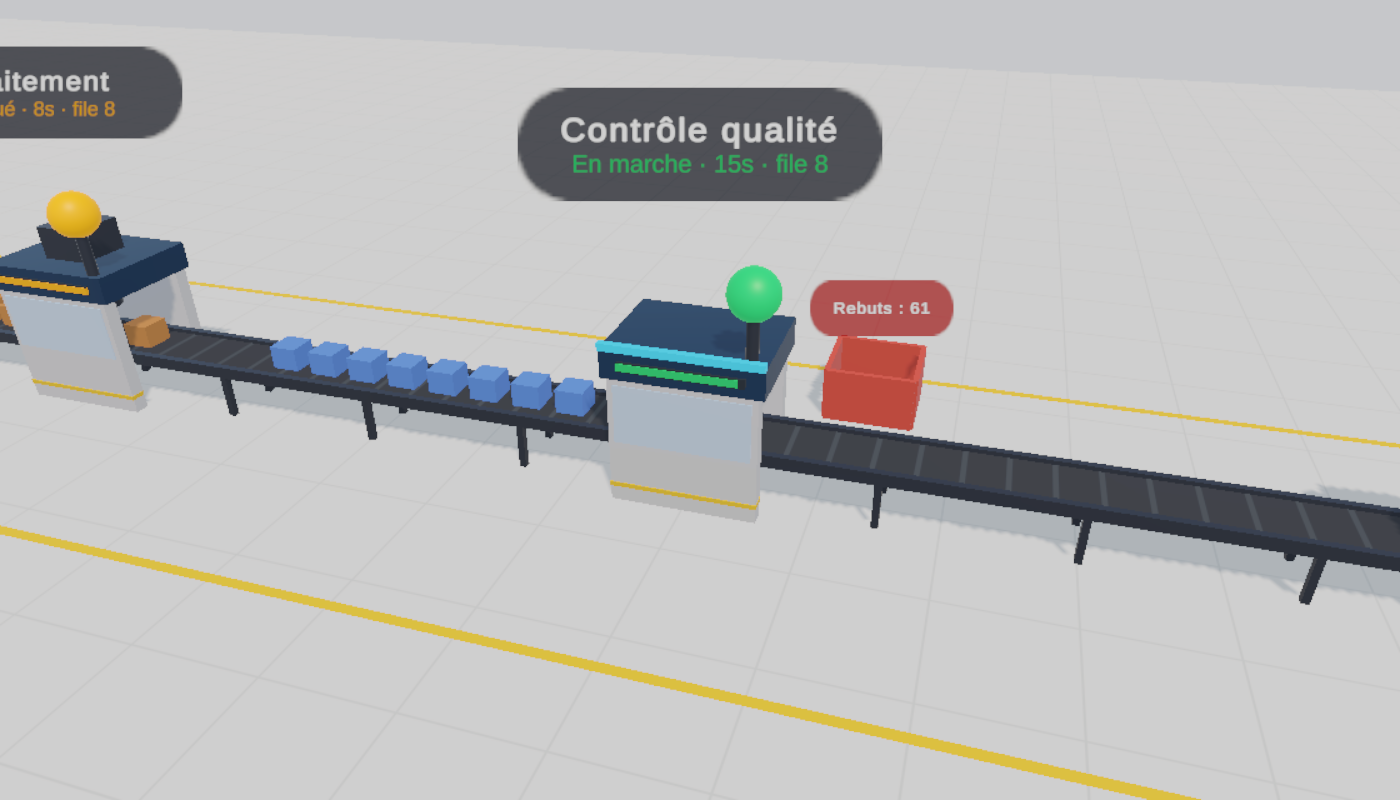
\includegraphics[width=\textwidth]{images/screenshots/zoom_controle.png}
  \caption{Zoom sur une machine~: étiquette d'état, voyant et barre de progression.}
\end{subfigure}\hfill
\begin{subfigure}[t]{0.49\textwidth}
  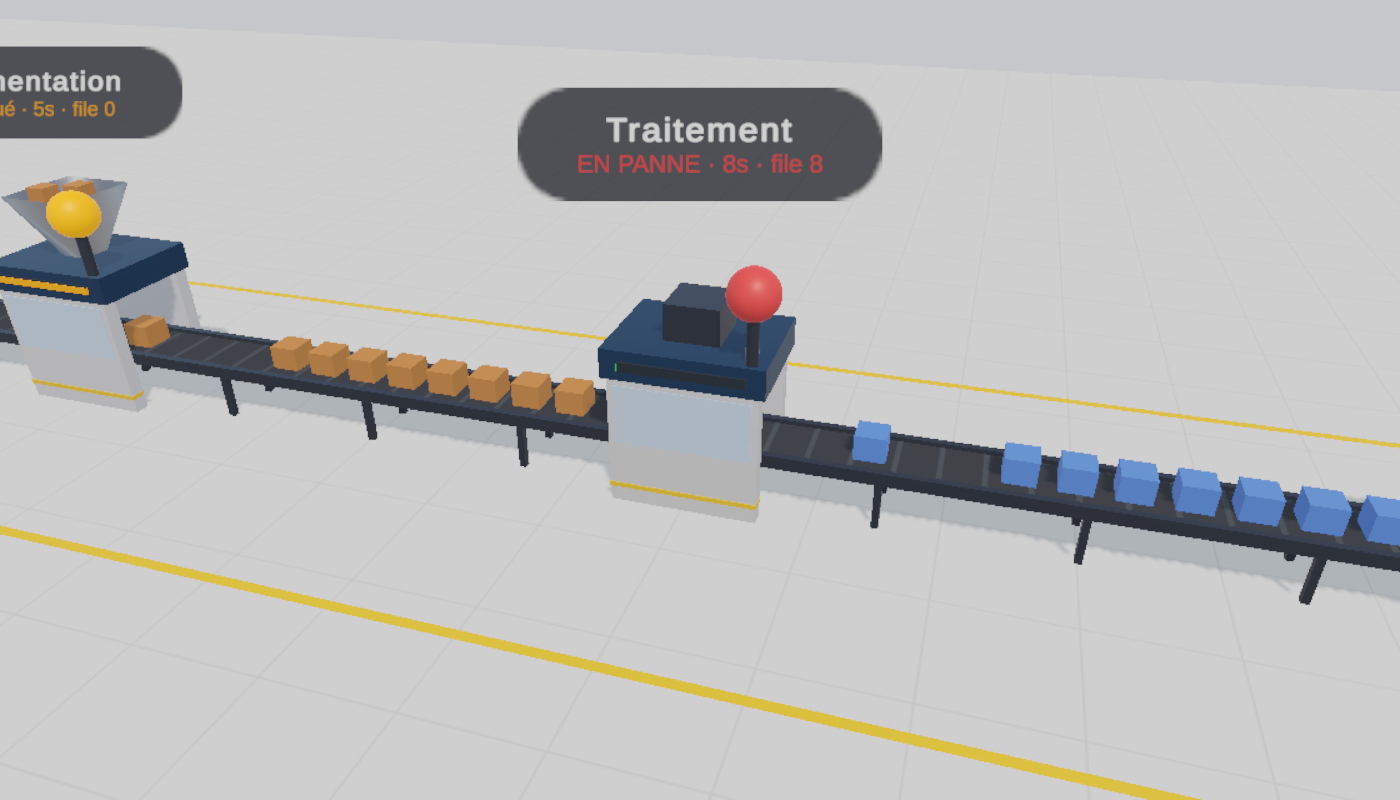
\includegraphics[width=\textwidth]{images/screenshots/panne_traitement.png}
  \caption{Panne provoquée sur le traitement~: voyant rouge, file amont pleine.}
\end{subfigure}
\caption{États visuels dans la scène Unity.}
\label{fig:etats_3d}
\end{figure}

\section{Le tableau de bord (\code{app.js})}

Le panneau latéral comporte trois onglets. \textbf{Supervision} affiche les \ac{KPI}, le tableau des postes, la courbe de débit des trois dernières minutes avec le débit théorique, les réglages du scénario, la fiche de la machine sélectionnée (\ac{MTBF}, \ac{MTTR}, disponibilité) et le journal. \textbf{Historique} relit la base SQLite par l'\ac{API} \ac{REST}. \textbf{Aide} résume la prise en main.

\begin{figure}[H]
\centering
\begin{subfigure}[t]{0.32\textwidth}
  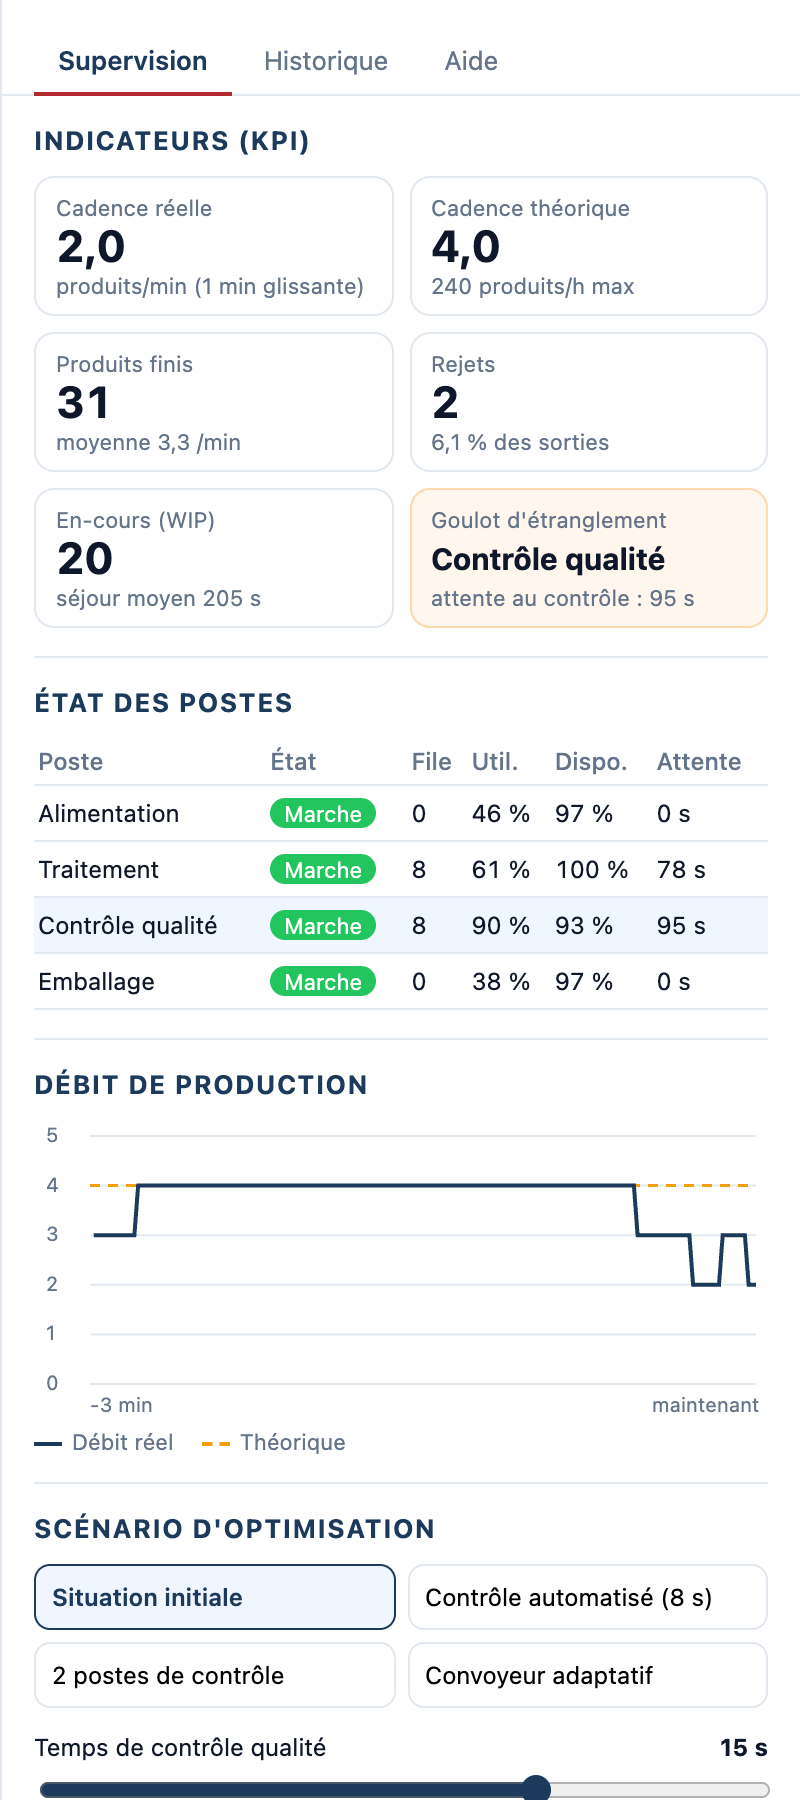
\includegraphics[width=\textwidth]{images/screenshots/dashboard_kpi.png}
  \caption{Supervision.}
\end{subfigure}\hfill
\begin{subfigure}[t]{0.32\textwidth}
  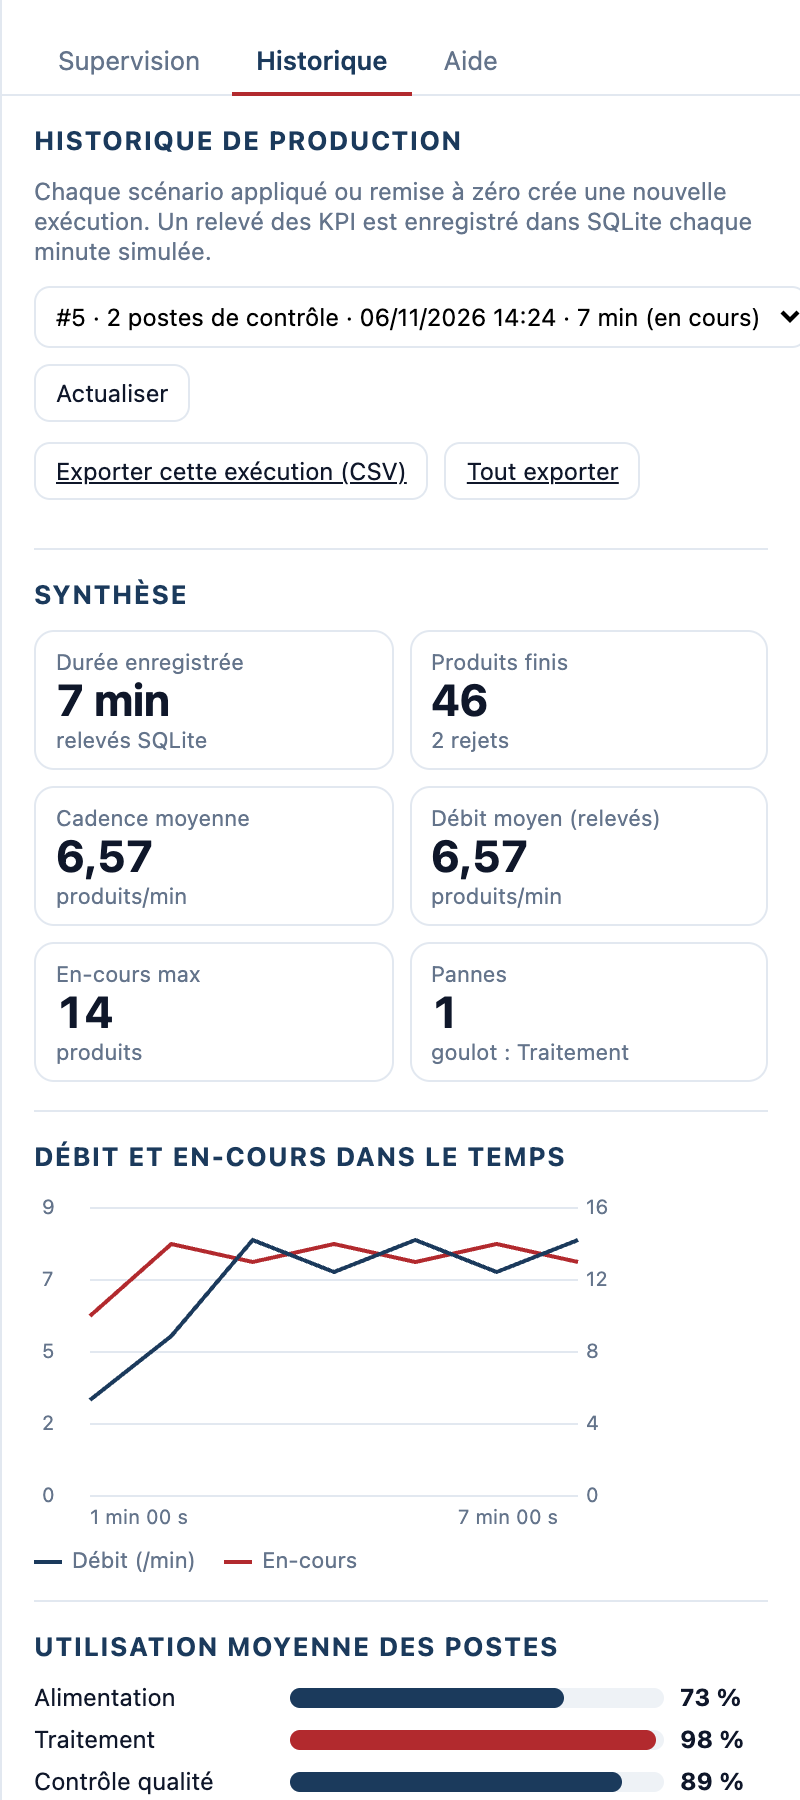
\includegraphics[width=\textwidth]{images/screenshots/historique.png}
  \caption{Historique (SQLite).}
\end{subfigure}\hfill
\begin{subfigure}[t]{0.32\textwidth}
  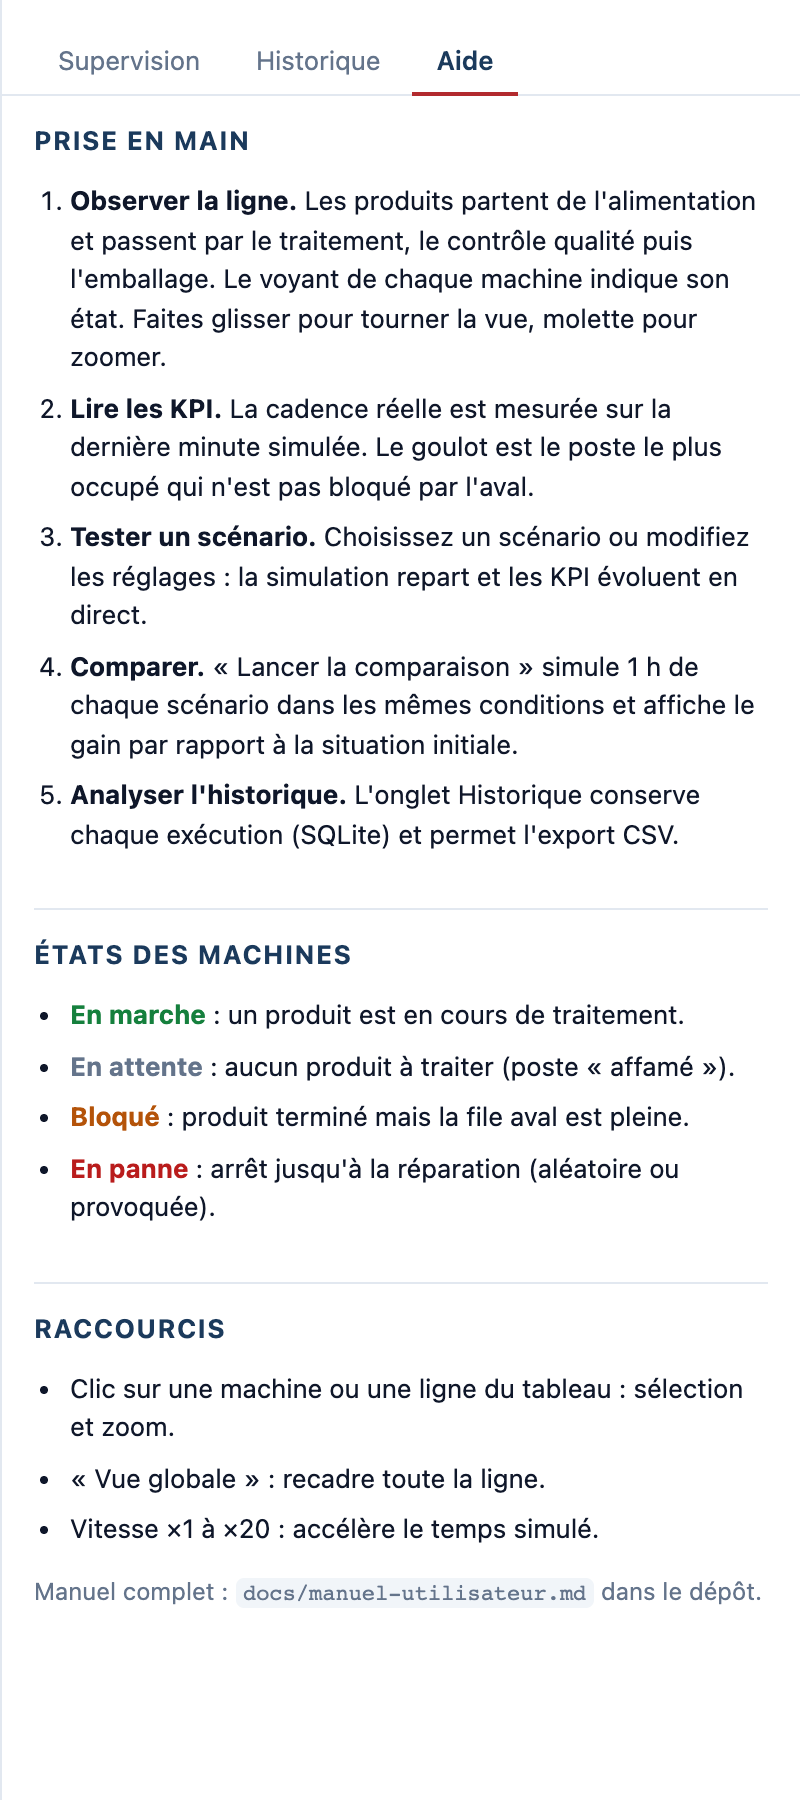
\includegraphics[width=\textwidth]{images/screenshots/aide.png}
  \caption{Aide.}
\end{subfigure}
\caption{Les trois onglets du tableau de bord.}
\label{fig:dashboard}
\end{figure}

\section{Validation du modèle}

Mohamed \textsc{Hamdouch} étant responsable de la validation, le modèle est vérifié par \textbf{23 tests automatisés} (pytest), exécutés en moins d'une minute. Ils ne vérifient pas que le code \enquote{tourne}, mais que la simulation respecte des propriétés connues d'une ligne de production~:

\begin{table}[H]
\centering
\caption{Propriétés vérifiées par les tests automatisés.}
\label{tab:tests}
\begin{tabularx}{\textwidth}{@{}X l@{}}
\toprule
\textbf{Propriété vérifiée} & \textbf{Résultat} \\
\midrule
Débit de régime (sans pannes ni rejets) égal au débit théorique à 5~\% près~: 4,0 / 7,5 / 7,5 produits/min & 3/3 \\
Conservation~: produits créés = finis + rejetés + en-cours, pour chaque scénario & 4/4 \\
Aucune file ne dépasse sa capacité (8, ou 3 en mode adaptatif) & 4/4 \\
Utilisation et disponibilité comprises entre 0 et 1 & 1/1 \\
Les pannes réduisent la disponibilité et la production~; une panne provoquée arrête le poste & 2/2 \\
Taux de rejet observé proche de 5~\% sur 4~h simulées & 1/1 \\
Le goulot est identifié au contrôle, puis déplacé au traitement après optimisation & 1/1 \\
Le convoyeur adaptatif réduit l'en-cours sans perte de débit & 1/1 \\
Comparaison reproductible à graine identique~; ajout et retrait de machines sans perte de produit & 2/2 \\
Historique~: relevés, événements, export \ac{CSV}~; \ac{API} \ac{WS} et \ac{REST} & 4/4 \\
\midrule
\textbf{Total} & \textbf{23/23} \\
\bottomrule
\end{tabularx}
\end{table}

Un contrôle supplémentaire est fourni par la \textbf{loi de Little}~\cite{little1961}, $L = \lambda W$~: l'en-cours moyen doit égaler le débit d'entrée multiplié par le temps de séjour moyen. Sur la ligne initiale avec pannes, $\lambda = (218 + 12)/3600$~produits/s et $W = 286$~s donnent $L \approx 18{,}3$, pour un en-cours moyen mesuré de 19{,}0. L'écart de 4~\% s'explique par les produits encore en ligne en fin de simulation, dont le séjour n'est pas compté dans $W$.
